\documentclass{beamer}

\usetheme[]{Madrid}
\usepackage[symbol]{footmisc}

\title{A Brief History of Computing}
\author{Will Leeson}
\date{January 24th, 2023}

\begin{document}

\begin{frame}
    \titlepage
\end{frame}

\begin{frame}
    \frametitle{What is a computer?}
    \begin{alertblock}<1->{Definition - Computer}
        A programmable, usually electronic, device that can store, retrieve, and process data\cite{mw:computer}
    \end{alertblock}
    \begin{block}<2>{Origin}
        The first use of the term comes from human ``computers''.
    \end{block}
\end{frame}

\begin{frame}
    \frametitle{Pre-20th Century - Generic Computers}
    \begin{columns}
        \begin{column}{0.5\linewidth}
            \begin{itemize}
                \item Recording Information
                \begin{itemize}
                    \item Tally Stick
                    \item Marked Cloth
                \end{itemize}
                \item Processing Information
                \begin{itemize}
                    \item Abacus
                    \item Slide Rule
                \end{itemize}
            \end{itemize}
        \end{column}
        \begin{column}{0.5\linewidth}
            \centering
            \includegraphics<1->[width=\linewidth]{tally-stick.jpeg}
            \includegraphics<2>[width=0.9\linewidth]{Abacus.png}
        \end{column}
    \end{columns}
\end{frame}

\begin{frame}
    \frametitle{Mechanical Computers}
    \begin{columns}
        \begin{column}{0.6\linewidth}
            \begin{itemize}
                \item<1-> Charles Babbage (1791-1871)
                \begin{itemize}
                    \item<2-> The ``Father of the Computer''
                    \item<3-> Conceptualized a machine able to do generic computations
                    \item<4-> Programmed using punch cards
                    \item<5-> Involved actual moving parts and cranks
                \end{itemize} 
                \item<6-> Analog Computers
                \begin{itemize}
                    \item<7-> Used for scientific purposes
                    \item<8-> Had specific purposes: Solving Calculus problems, predicting tides, etc.
                \end{itemize}
            \end{itemize}
        \end{column}
        \begin{column}{0.4\linewidth}
            \centering
            \includegraphics<5->[width=\linewidth]{Babbage_Difference_Engine.jpg}
            \includegraphics<8->[width=\linewidth]{tide-prediction.jpg}
        \end{column}
    \end{columns} 
\end{frame}

\begin{frame}
    \frametitle{First Fully Electric computers}
    \begin{columns}
        \begin{column}{0.6\linewidth}
            \begin{itemize}
                \item<1-> Large devices that took up entire rooms
                \item<2-> Used Vacuum Tubes, which were prone to break
                \item<3-> Programmed to perform various functions 
            \end{itemize}
        \end{column}
        \begin{column}{0.4\linewidth}
            \centering
            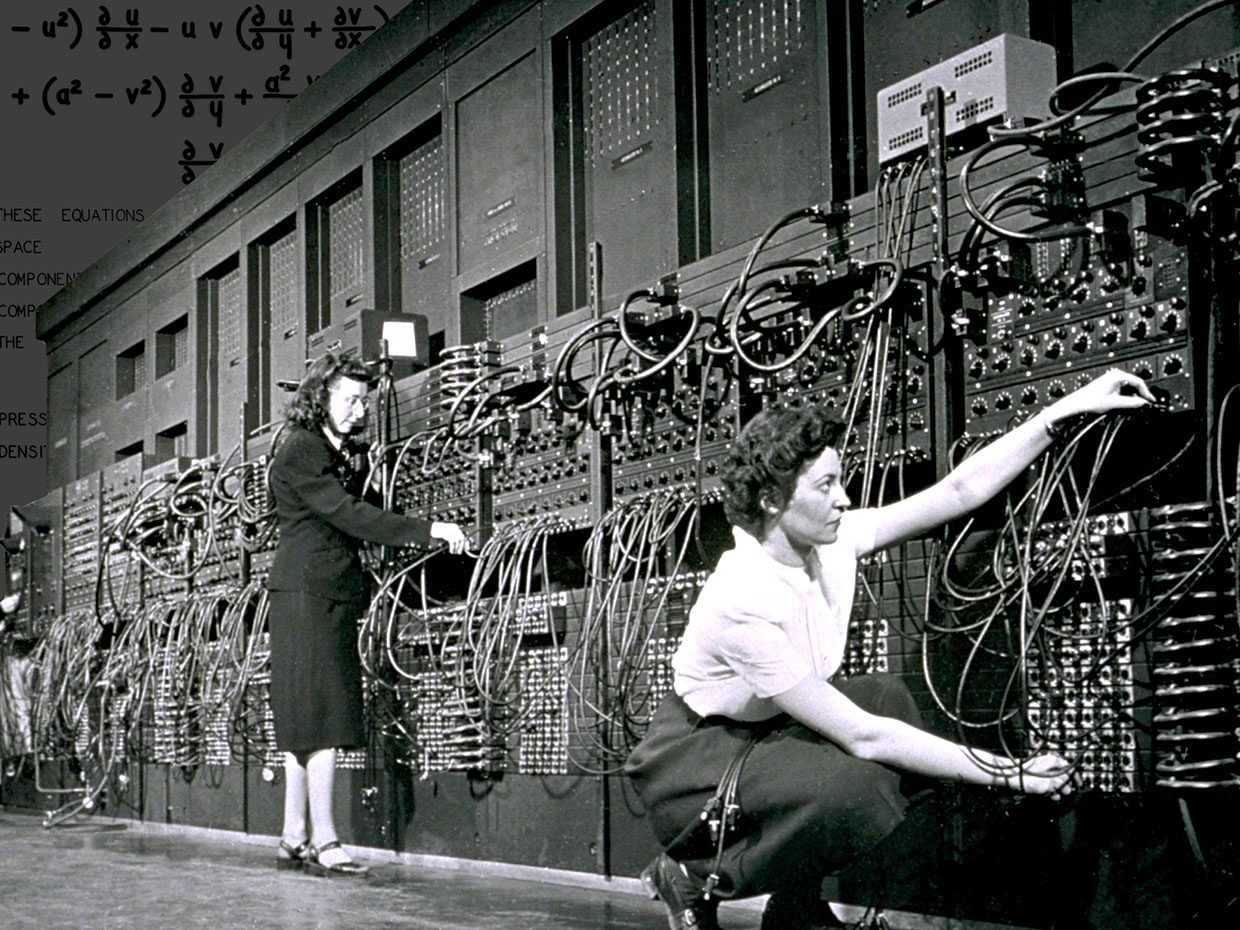
\includegraphics[width=\linewidth]{eniac.jpg}
        \end{column}
    \end{columns} 
\end{frame}

\begin{frame}
    \frametitle{Alan Turing}
    \begin{columns}
        \begin{column}{0.6\linewidth}
            \begin{itemize}
                \item<1-> Key figure in computing, cryptography, and artificial intelligence
                \item<2-> Helped break German ``Enigma'' in WWII
                \item<3-> Created the Turing Test and Turing Machine
            \end{itemize}
        \end{column}
        \begin{column}{0.4\linewidth}
            \centering
            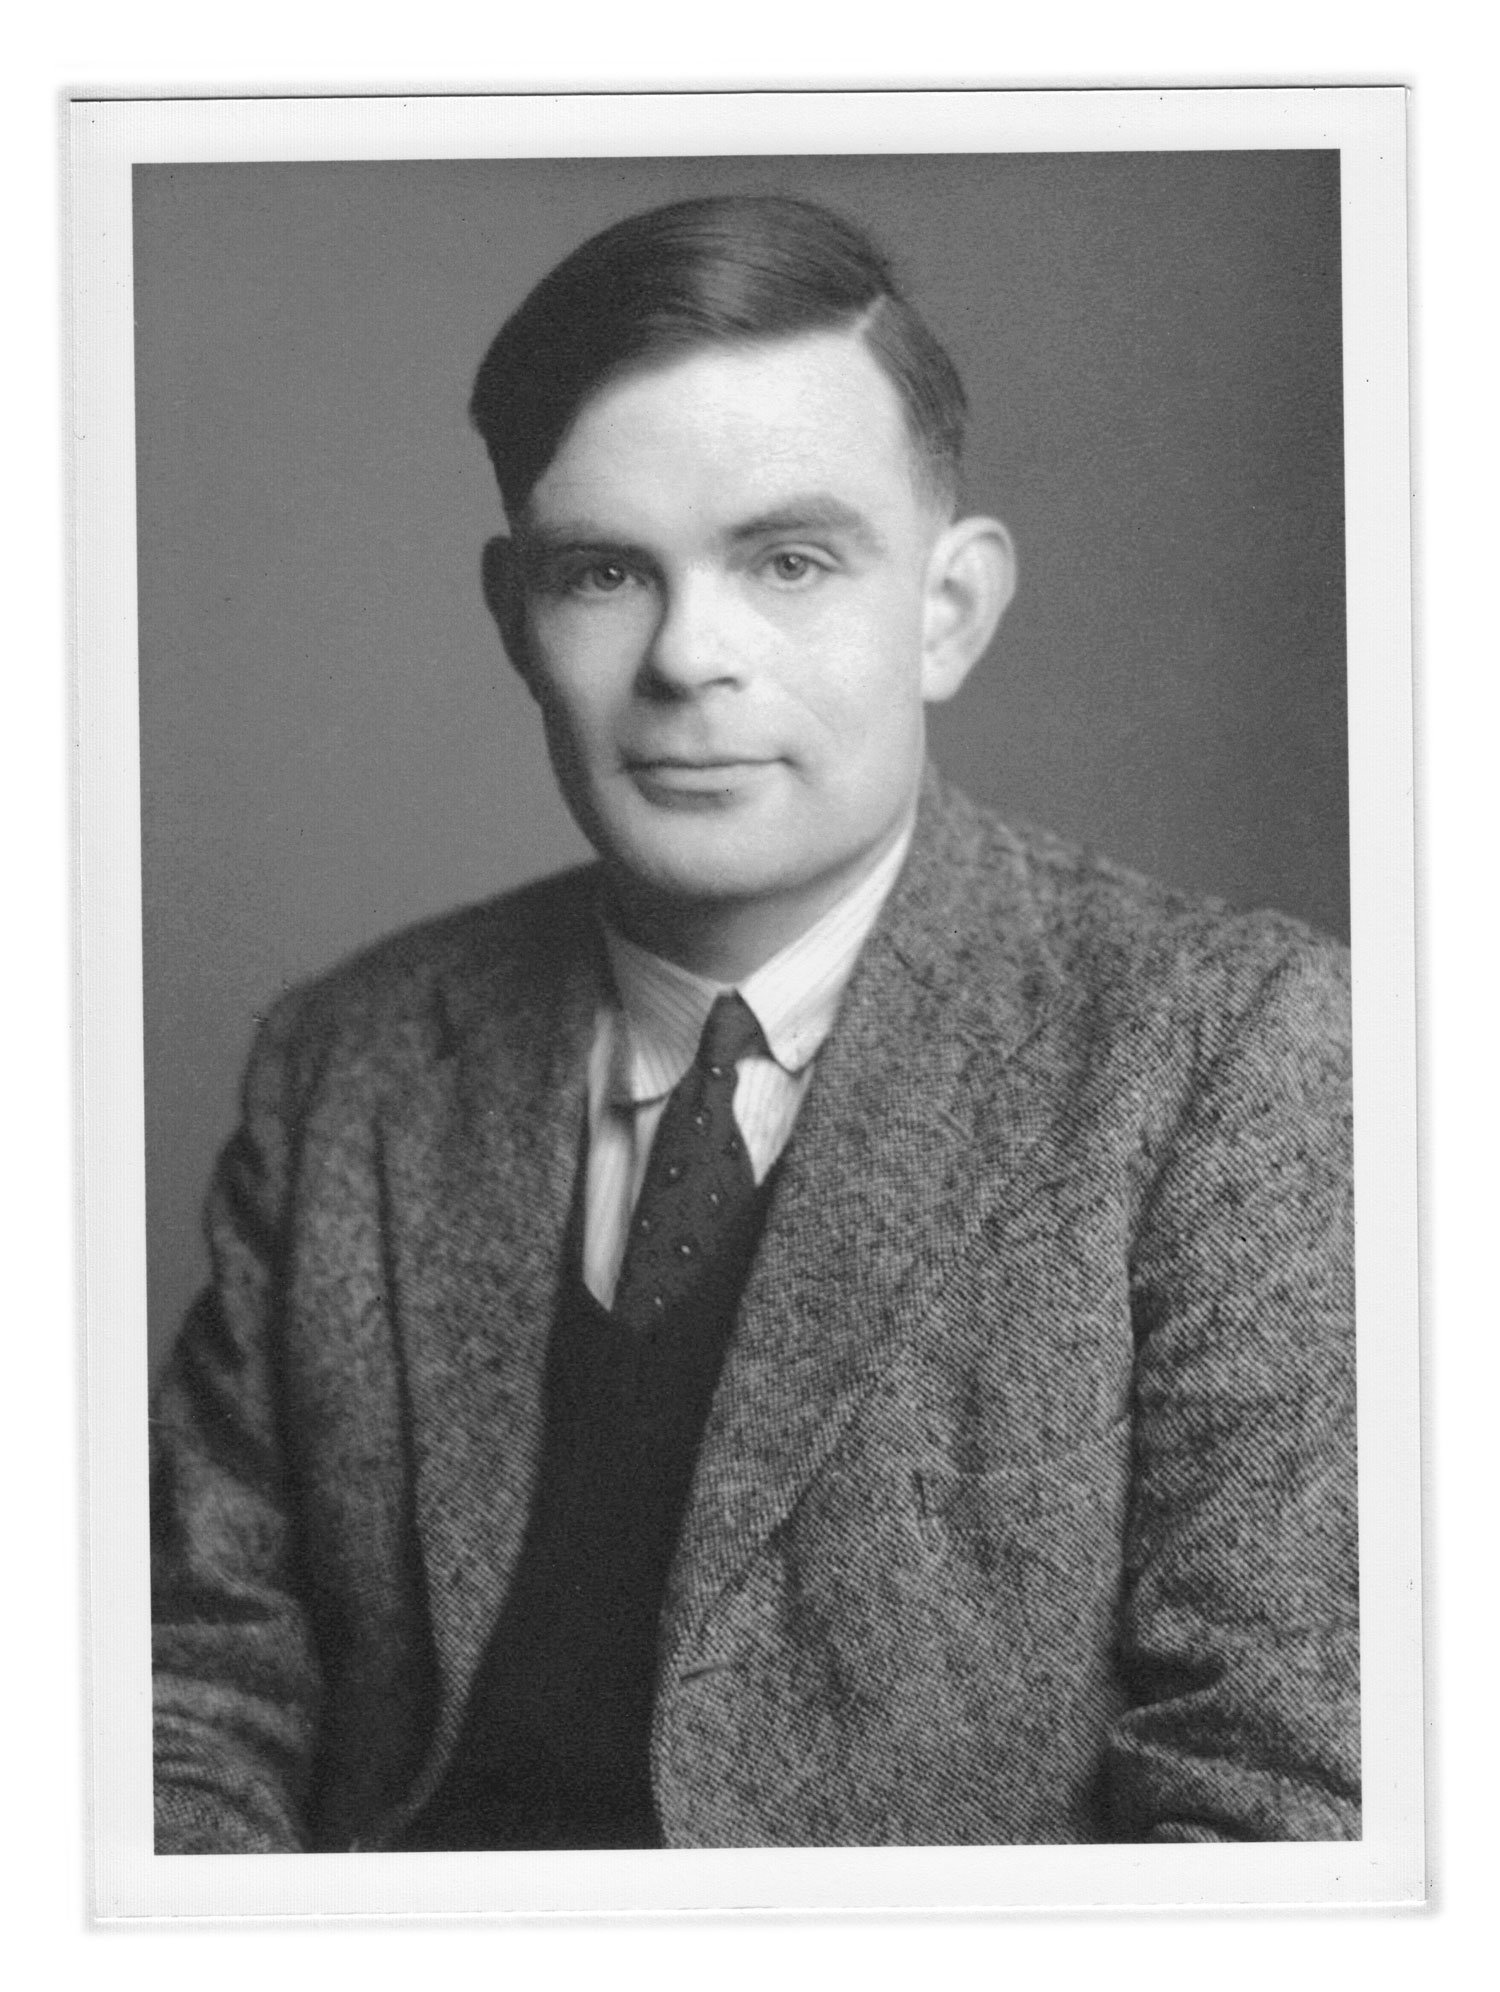
\includegraphics[width=\linewidth]{Alan_Turing.jpg}
        \end{column}
    \end{columns} 
\end{frame}

\begin{frame}
    \frametitle{Turing Machine}
    \begin{columns}
        \begin{column}{0.6\linewidth}
            \begin{itemize}
                \item<1-> A programmable machine capable of executing any algorithm
                \item<2-> Basis of modern computers 
                \item<3-> Proved both the power and limitations of computers
            \end{itemize}
        \end{column}
        \begin{column}{0.4\linewidth}
            \centering
            \includegraphics<3->[width=\linewidth]{turing-machine.png}
        \end{column}
    \end{columns} 
\end{frame}

\begin{frame}
    \frametitle{Programming Languages}
    \begin{columns}
        \begin{column}{0.6\linewidth}
            \begin{itemize}
                \item<1-> Speaking to a computer is difficult
                \item<3-> What we need is a translator
                \item<4-> Compilers are translators
            \end{itemize}
        \end{column}
        \begin{column}{0.4\linewidth}
            \centering
            \includegraphics<2>[width=\linewidth]{Binary_multiplier.png}
            \includegraphics<3>[width=\linewidth]{Translator.png}
            \includegraphics<4->[width=\linewidth]{Translator2.png}
        \end{column}
    \end{columns} 
\end{frame}

\begin{frame}[allowframebreaks]{Citations}
    \bibliography{citations.bib}
    \bibliographystyle{ieeetr}
\end{frame}

\end{document}